\documentclass{article}
\usepackage{geometry}
\geometry{margin=1in}
\usepackage{parskip}
\usepackage[most]{tcolorbox}
\usepackage{amsmath, amssymb}
\usepackage{tikz}
\usetikzlibrary{shapes, arrows.meta, positioning, shadows, fit, calc}

\title{Cybersecurity (CSCI 2413): Mid-Term Review Companion Guide}
\author{Elite Academic Professor}
\date{\today}
\begin{document}
\maketitle
\tableofcontents
\newpage

\section{OSINT (Open-Source Intelligence)}

\begin{tcolorbox}[title=Key Definition: OSINT]
\textbf{Open-Source Intelligence (OSINT)} refers to the systematic process of collecting, analyzing, and acting upon publicly available information to gather actionable insight and intelligence regarding a specific target. This practice is foundational in threat intelligence and the initial reconnaissance phase of security auditing.
\end{tcolorbox}

The term emphasizes the use of data that can be legally and ethically accessed by anyone, circumventing the need for covert measures. Crucially, the sources utilized for OSINT are incredibly diverse, covering almost any material released to the public domain.

\subsection{The OSINT Ecosystem}
The types of information sources that contribute to OSINT can be visualized as a comprehensive ecosystem, ranging from traditional media to private professional networks.

\begin{figure}[h]
    \centering
    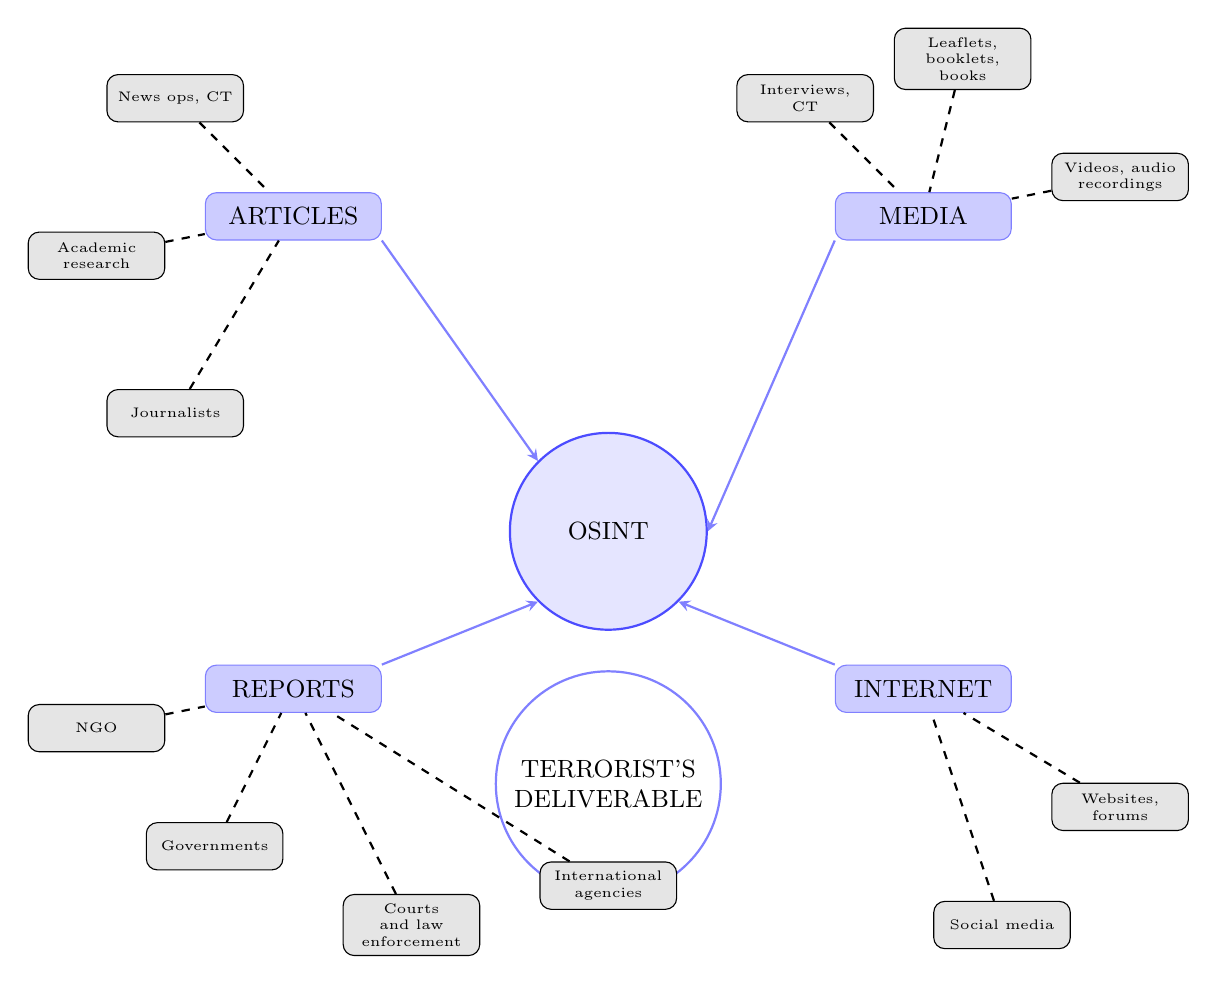
\begin{tikzpicture}[
        node distance=0.8cm, 
        font=\small, 
        main circle/.style={draw=blue!70, thick, circle, minimum size=2.5cm, align=center, fill=blue!10},
        inner circle/.style={draw=blue!50, thick, circle, minimum size=1.5cm, align=center, fill=white},
        category node/.style={draw=blue!50, rounded corners, align=center, fill=blue!20, minimum width=2cm, text width=2cm, minimum height=0.6cm},
        source node/.style={draw=black, rounded corners, align=center, fill=gray!20, minimum width=1.5cm, text width=1.5cm, minimum height=0.6cm, font=\tiny},
        arc arrow/.style={->, >=stealth, thick, blue!50}
    ]

    % Central Nodes
    \node[main circle] (osint) {OSINT};
    \node[inner circle, below=0.5cm of osint, text width=2.5cm, font=\small] (deliverable) {TERRORIST'S DELIVERABLE};

    % Outer Ring (Categories)
    \node[category node] (media) at (4, 4) {MEDIA};
    \node[category node] (internet) at (4, -2) {INTERNET};
    \node[category node] (reports) at (-4, -2) {REPORTS};
    \node[category node] (articles) at (-4, 4) {ARTICLES};

    % Specific Sources
    % Media (Top Right)
    \node[source node] (interviews) at (2.5, 5.5) {Interviews, CT};
    \node[source node] (leaflets) at (4.5, 6) {Leaflets, booklets, books};
    \node[source node] (videos) at (6.5, 4.5) {Videos, audio recordings};
    
    % Internet (Bottom Right)
    \node[source node] (websites) at (6.5, -3.5) {Websites, forums};
    \node[source node] (social) at (5, -5) {Social media};
    
    % Reports (Bottom Left)
    \node[source node] (agencies) at (0, -4.5) {International agencies};
    \node[source node] (courts) at (-2.5, -5) {Courts and law enforcement};
    \node[source node] (governments) at (-5, -4) {Governments};
    \node[source node] (ngo) at (-6.5, -2.5) {NGO};

    % Articles (Top Left)
    \node[source node] (journalists) at (-5.5, 1.5) {Journalists};
    \node[source node] (academic) at (-6.5, 3.5) {Academic research};
    \node[source node] (news) at (-5.5, 5.5) {News ops, CT};

    % Connect the outer categories to the center (simplified direct connections)
    \draw[arc arrow] (media.south west) -- (osint.east);
    \draw[arc arrow] (internet.north west) -- (osint.south east);
    \draw[arc arrow] (reports.north east) -- (osint.south west);
    \draw[arc arrow] (articles.south east) -- (osint.north west);

    % Connect sources to categories (implied grouping)
    \draw[thick, dashed] (interviews) -- (media);
    \draw[thick, dashed] (leaflets) -- (media);
    \draw[thick, dashed] (videos) -- (media);
    
    \draw[thick, dashed] (websites) -- (internet);
    \draw[thick, dashed] (social) -- (internet);

    \draw[thick, dashed] (agencies) -- (reports);
    \draw[thick, dashed] (courts) -- (reports);
    \draw[thick, dashed] (governments) -- (reports);
    \draw[thick, dashed] (ngo) -- (reports);

    \draw[thick, dashed] (journalists) -- (articles);
    \draw[thick, dashed] (academic) -- (articles);
    \draw[thick, dashed] (news) -- (articles);
    
    \end{tikzpicture}
    \caption{The Diverse Sources Contributing to Open-Source Intelligence}
\end{figure}

\newpage

\section{The OSINT Workflow}

The collection and analysis of open-source intelligence typically follows a structured, cyclical process composed of several key phases:

\subsection{Planning and Direction}
This initial phase is critical for success. It requires establishing clear objectives, often driven by intelligence requirements. Analysts must precisely define what information is needed and, critically, why it is needed, ensuring that subsequent efforts are targeted and efficient.

\subsection{Collection}
This stage involves the actual gathering of raw data from public sources. This includes social media monitoring, scanning public records (such as property or court documents), reviewing news archives, and utilizing deep web search tools. The collection process employs both manual techniques (human searching) and automated methods (scrapers, APIs) to maximize data acquisition.

\subsection{Processing and Organization}
Raw collected data is voluminous and often messy. Processing involves filtering this data to retain only relevant information pertinent to the established objectives. Duplicate entries must be removed, and the data is often structured or indexed. This stage remains highly manual, as human expertise is needed to contextualize and validate the sources.

\subsection{Analysis and Correlation}
During analysis, the processed data is examined to identify patterns, emerging relationships, and defining trends. A crucial component is correlation, where findings are cross-referenced and corroborated using multiple independent sources to ensure accuracy and reduce the risk of relying on disinformation or single points of failure. This validation process transforms raw data into actionable intelligence.

\subsection{Dissemination}
The final phase involves reporting the verified findings to the relevant stakeholders, who might be internal security teams, external clients, or management. The report must be delivered in a structured, coherent way, typically taking the form of a formal report, a detailed briefing, or an alert notification.

\newpage

\section{OSINT Targets and Applications}

OSINT techniques are applied across various domains for reconnaissance, threat intelligence, and risk assessment. Common targets include:

\subsection{Individuals}
Investigating individuals often involves social media intelligence (SOCMINT), identifying personal networks, behavioral patterns, and associated risks. For instance, a background check or assessment of an employee's external activities falls under this category.

\subsection{Organizations and Businesses}
For corporate entities, OSINT can reveal organizational structure, partnerships, technological footprints, public financial filings, and supply chain vulnerabilities. This information is vital for competitive intelligence and penetration testing reconnaissance.

\subsection{Critical Infrastructure}
This involves gathering public information related to essential services like power grids, water supply, and transportation networks. Such reconnaissance helps identify weaknesses that could be exploited by adversaries, allowing defenders to preemptively harden systems.

\subsection{Cybersecurity and Threat Intelligence}
OSINT is a core component of threat intelligence, used to monitor forums, dark web activity (where accessible publicly), and security blogs to track new attack vectors, malware campaigns, and threat actors.

\subsection{Governments and Nations}
This involves collecting publicly available governmental documents, policy statements, legislative debates, and open-source military data to inform strategic decision-making and foreign policy analysis.

\subsection{Public Health}
In public health, OSINT is used for tracking disease outbreaks, monitoring public reaction to health policies, and identifying regional resource deficits by analyzing publicly shared reports and data.

\newpage

\section{Sock Puppet Accounts and SOCMINT}

\begin{tcolorbox}[title=Key Definition: Sock Puppet]
A \textbf{Sock Puppet} is a covert online account or identity utilized by an investigator that is deliberately not related to their true personal or professional identity.
\end{tcolorbox}

The primary purpose of using a sock puppet account in intelligence gathering, especially within the scope of Social Media Intelligence (\textbf{SOCMINT}), is anonymity. By using a fabricated identity, the analyst protects their true identity from being revealed to the target or other associated parties. This protection is essential to avoid burning the identity of the analyst or compromising the investigation.

When conducting such operations, it is crucial to maximize operational security (OPSEC). Best practices dictate isolating the investigative environment entirely:
\begin{itemize}
    \item \textbf{Virtual Machine (VM):} Operations should be conducted from a Virtual Machine (VM). This isolates the activities from the analyst's primary operating system, creating a clean, disposable environment that minimizes the risk of infection or leakage.
    \item \textbf{VPN (Virtual Private Network):} Using a VPN ensures that the physical location and the network IP address of the analyst are masked, preventing geographical tracking and IP-based attribution by the target or platform providers.
\end{itemize}
These measures ensure that the only trace left behind belongs to the constructed sock puppet identity.

\newpage

\section{Cryptography Basics}

Cryptography is the practice and study of techniques for secure communication in the presence of adversarial behavior. It primarily deals with two processes: encryption and decryption.

\subsection{Encryption}
Encryption is the method by which plain text (readable data) is transformed into cipher text (unreadable, scrambled data).
\begin{itemize}
    \item \textbf{Algorithm:} An algorithm is utilized to scramble the plain text based on a specific set of rules and a key.
    \item \textbf{Shared Protocol:} For successful communication, the sender and receiver must agree on the specific algorithm being used.
    \item \textbf{Security:} Without knowing the correct protocol and key, the resulting message is computationally difficult to reverse-engineer back into the original plain text.
\end{itemize}

\subsection{Decryption}
Decryption is the complementary process, involving the reversal of the scrambling protocol (the encryption algorithm) using the correct key. This process transforms the cipher text back into the original comprehensible plain text message.

\subsection{Sample Encryption and Decryption Process}

% \begin{figure}[h]
%     \centering
%     \begin{tikzpicture}[
%         node distance=1.5cm,
%         block/.style={rectangle, draw, thick, text width=2cm, align=center, minimum height=1cm, rounded corners, fill=white},
%         data/.style={rectangle, draw, thick, text width=2.5cm, align=center, minimum height=1.5cm, rounded corners, fill=gray!10},
%         process/.style={circle, draw, thick, minimum size=0.5cm, fill=white},
%         key_icon/.style={draw, thick, fill=yellow!30, minimum size=0.5cm, shape=coordinate}, % Placeholder for complex key visual
%         arrow/.style={->, >=stealth, thick},
%         box_style/.style={rectangle, draw, fill=blue!20, text width=8cm, align=center, inner sep=5pt}
%     ]
    
%     \node[box_style] (title) {SAMPLE ENCRYPTION AND DECRYPTION PROCESS};

%     % Encryption Row
%     \node[data, below=1.5cm of title, xshift=-4cm] (plain_e) {Plain Text};
%     % \node[block, left=1cm of plain_e, text width=1cm] (label_e) {Encryption};
%     \node[process, right=1.5cm of plain_e] (plus_e) {+};
%     \node[process, right=1.5cm of plus_e] (dot_e) {$\dots$};
%     \node[block, right=1.5cm of dot_e] (algo_e) {Algorithm};
%     \node[process, right=1.5cm of algo_e] (dot2_e) {$\dots$};
%     \node[data, right=1.5cm of dot2_e] (cipher_e) {Cipher Text};
    
%     % Key source
%     \node[draw=none, above=0.3cm of plain_e] (key_paper_e) {\tiny SSN 789-43-1658};
%     \node[key_icon, above=0.3cm of plus_e] (KeyE) {};
%     \draw[arrow] (plain_e) -- (plus_e);
%     \draw[arrow] (plus_e) -- (dot_e);
%     \draw[arrow] (dot_e) -- (algo_e);
%     \draw[arrow] (algo_e) -- (dot2_e);
%     \draw[arrow] (dot2_e) -- (cipher_e);
    
%     % Cipher text sample
% %     \node[draw=none, above=0.3cm of cipher_e] (cipher_data) {\tiny BBK\\ 4d9yt0op\\ FDR2NC$\dots$};

% %     % Decryption Row
% %     \node[data, below=4.5cm of title, xshift=-4cm] (cipher_d) {Cipher Text};
% %     \node[block, left=1cm of cipher_d, text width=1cm] (label_d) {Decryption};
% %     \node[process, right=1.5cm of cipher_d] (plus_d) {+};
% %     \node[process, right=1.5cm of plus_d] (dot_d) {$\dots$};
% %     \node[block, right=1.5cm of dot_d] (algo_d) {Algorithm};
% %     \node[process, right=1.5cm of algo_d] (dot2_d) {$\dots$};
% %     \node[data, right=1.5cm of dot2_d] (plain_d) {Plain Text};

% %     % Key source for Decryption
% %     \node[key_icon, above=0.3cm of plus_d] (KeyD) {};
% %     \draw[arrow] (cipher_d) -- (plus_d);
% %     \draw[arrow] (plus_d) -- (dot_d);
% %     \draw[arrow] (dot_d) -- (algo_d);
% %     \draw[arrow] (algo_d) -- (dot2_d);
% %     \draw[arrow] (dot2_d) -- (plain_d);
    
% %     % Plain text output
% %     \node[draw=none, above=0.3cm of plain_d] (key_paper_d) {\tiny SSN 789-43-1658};
    
% %     % Visualizing the Key
% %     \node[draw=black, thick, rotate=45, minimum size=0.5cm, fill=gray!30] at ($(KeyE)+(0.25cm, 0.25cm)$) {};
% %     \node[draw=black, thick, rotate=45, minimum size=0.5cm, fill=gray!30] at ($(KeyD)+(0.25cm, 0.25cm)$) {};


%     \end{tikzpicture}
%     \caption{Encryption and Decryption Flow}
% \end{figure}

\newpage

\section{Cryptography Basics (Continued)}

Cryptographic ciphers are traditionally categorized based on how they manipulate the plain text:

\subsection{Transposition Ciphers}
Transposition ciphers rearrange the order of the letters in the plain text without changing the letters themselves. Intuitively, this is like shuffling a deck of cards; the cards remain the same, but their sequence is altered.

\subsection{Substitution Ciphers}
Substitution ciphers systematically replace each letter or group of letters in the plain text with a different letter, number, or symbol.

\subsubsection{Types of Substitution}
Substitution methods are further classified based on key management:
\begin{enumerate}
    \item \textbf{Single/Symmetric Key Encryption:} This uses the same secret key for both encryption and decryption.
    \begin{itemize}
        \item \textbf{Stream Ciphers:} Encrypt one bit or byte of plain text at a time.
        \item \textbf{Block Ciphers:} Encrypt a fixed-size block of bits simultaneously (e.g., 64-bit or 128-bit blocks).
    \end{itemize}
    \item \textbf{Public/Asymmetric Key Encryption:} This uses a pair of mathematically related keys: a public key for encryption and a private key for decryption.
\end{enumerate}

\newpage

\section{Transposition Ciphers: The Rail Fence}

A classic example of a transposition cipher is the Rail Fence cipher, which writes the plain text downwards on successive "rails" and then reads the result off row by row.

\subsection{Example: Rail Fence Encryption}
Consider the message: \textbf{``Defend the east wall''} with a \textbf{key of 3} (meaning 3 rails). Spaces are removed and the plaintext is $D E F E N D T H E E A S T W A L L X$ (19 characters).

\begin{figure}[h]
    \centering
    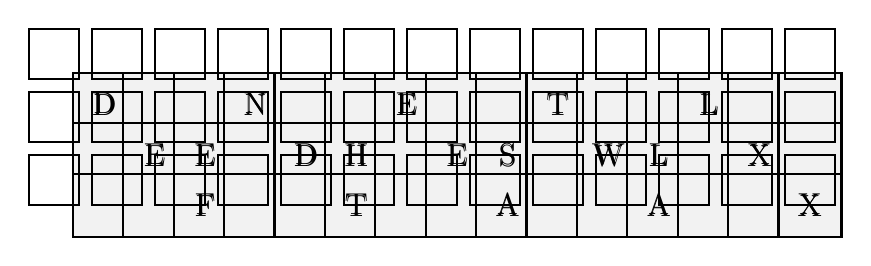
\begin{tikzpicture}[scale=0.8, cell/.style={rectangle, draw=black, minimum size=0.8cm, thick, align=center, fill=gray!10}]

        % Draw the grid and labels
        \foreach \i in {1,...,3} {
            \foreach \j in {1,...,15} {
                \node[cell] at (\j*0.8, -\i*0.8) (C-\i-\j) {};
            }
        }
        
        % Place letters based on slide visual:
        % Row 1: D N E T L
        \node at (C-1-1) {D}; \node at (C-1-4) {N}; \node at (C-1-7) {E}; \node at (C-1-10) {T}; \node at (C-1-13) {L};
        
        % Row 2: E E D H E S W L X
        \node at (C-2-2) {E}; \node at (C-2-3) {E}; \node at (C-2-5) {D}; \node at (C-2-6) {H}; \node at (C-2-8) {E}; \node at (C-2-9) {S}; \node at (C-2-11) {W}; \node at (C-2-12) {L}; \node at (C-2-14) {X};
        
        % Row 3: F T A A X
        \node at (C-3-3) {F}; \node at (C-3-6) {T}; \node at (C-3-9) {A}; \node at (C-3-12) {A}; \node at (C-3-15) {X};
        
        % Remove fill from empty cells for clarity
        \foreach \i in {1,...,3} {
            \foreach \j in {1,...,15} {
                \pgfmathtruncatemacro{\x}{\j*0.8}
                \pgfmathtruncatemacro{\y}{-\i*0.8}
                % Draw lines without filling background
                \draw[thick] (\x-0.4, \y-0.4) rectangle (\x+0.4, \y+0.4);
            }
        }
        
        % Re-add the letters (using the original coordinates which are centered)
        \node[font=\large] at (C-1-1) {D}; \node[font=\large] at (C-1-4) {N}; \node[font=\large] at (C-1-7) {E}; \node[font=\large] at (C-1-10) {T}; \node[font=\large] at (C-1-13) {L};
        
        \node[font=\large] at (C-2-2) {E}; \node[font=\large] at (C-2-3) {E}; \node[font=\large] at (C-2-5) {D}; \node[font=\large] at (C-2-6) {H}; \node[font=\large] at (C-2-8) {E}; \node[font=\large] at (C-2-9) {S}; \node[font=\large] at (C-2-11) {W}; \node[font=\large] at (C-2-12) {L}; \node[font=\large] at (C-2-14) {X};
        
        \node[font=\large] at (C-3-3) {F}; \node[font=\large] at (C-3-6) {T}; \node[font=\large] at (C-3-9) {A}; \node[font=\large] at (C-3-12) {A}; \node[font=\large] at (C-3-15) {X};

    \end{tikzpicture}
    \caption{Rail Fence Grid (Key=3)}
\end{figure}

The cipher text is generated by reading the content row by row, starting from the top rail:
\begin{center}
\Large
\textbf{DNETLEEDHESWLXFTAAX}
\end{center}

\newpage

\section{Transposition Cipher: Decryption Example}

Decryption of a Rail Fence cipher requires knowing the length of the message and the key (number of rails). The process involves reconstructing the fence pattern using placeholders and then mapping the cipher text back into the pattern.

Ciphertext: \textbf{TEKOOHRACIRMNREATANFTETYTGHH} \\
Length: 28 \\
Key: \textbf{4}

\subsection{Step 1: Determine Rail Lengths and Placement}
We map the 28 letters onto the 4-rail zig-zag pattern to determine where each letter of the ciphertext belongs.

\begin{figure}[h]
    \centering
    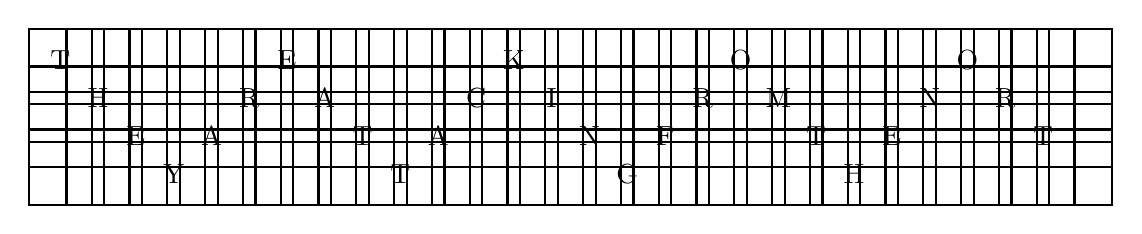
\begin{tikzpicture}[scale=0.6, cell/.style={rectangle, draw=black, minimum size=0.8cm, thick, align=center}]
        \def\gridrows{4}
        \def\gridcols{28}
        
        % Draw the grid and place markers 
        \foreach \i in {1,...,\gridrows} {
            \foreach \j in {1,...,\gridcols} {
                \node[cell] at (\j*0.8, -\i*0.8) (C-\i-\j) {};
            }
        }
        
        % Row 1 (5 letters: T E K O O)
        \node at (C-1-1) {T}; \node at (C-1-7) {E}; \node at (C-1-13) {K}; \node at (C-1-19) {O}; \node at (C-1-25) {O};
        
        % Row 2 (9 letters: H R A C I R M N R)
        \node at (C-2-2) {H}; \node at (C-2-6) {R}; \node at (C-2-8) {A}; \node at (C-2-12) {C}; \node at (C-2-14) {I}; \node at (C-2-18) {R}; \node at (C-2-20) {M}; \node at (C-2-24) {N}; \node at (C-2-26) {R};

        % Row 3 (10 letters: E A T A N F T E T)
        \node at (C-3-3) {E}; \node at (C-3-5) {A}; \node at (C-3-9) {T}; \node at (C-3-11) {A}; \node at (C-3-15) {N}; \node at (C-3-17) {F}; \node at (C-3-21) {T}; \node at (C-3-23) {E}; \node at (C-3-27) {T}; 
        
        % Row 4 (4 letters: Y T G H)
        \node at (C-4-4) {Y}; \node at (C-4-10) {T}; \node at (C-4-16) {G}; \node at (C-4-22) {H};
        
    \end{tikzpicture}
    \caption{Rail Fence Decryption Grid (Key=4)}
\end{figure}

\end{document}